In order to fit for anomalous couplings we used a maximum likelihood fit in
the RooFit framework. Differences between the Standard Model
and anomalous couplings are established in the leading lepton
\pt\ distribution and the overall \ww\ event yield. The combined PDF for the
leading lepton \pt\ distribution is:
\begin{equation}
  P(\pt) = \frac{N^\mathrm{exp}_\mathrm{sig}}{N^\mathrm{exp}}P_\mathrm{sig}(\pt) + 
  \frac{N^\mathrm{exp}_\mathrm{bkg}}{N^\mathrm{exp}}P_\mathrm{bkg}(\pt) 
\end{equation}
where $P_\mathrm{sig}$ and $P_\mathrm{bkg}$ are signal and background PDFs of the
leading lepton \pt{}, $N^\mathrm{exp}_\mathrm{sig}$ and $N^\mathrm{exp}_\mathrm{bkg}$ are the expected
number of signal and background events and
$N^\mathrm{exp}=N^\mathrm{exp}_\mathrm{sig}+N^\mathrm{exp}_\mathrm{bkg}$.

The Likelihood is defined as a product of Poisson PDFs for the observed
number of events and the combined PDF for each event:
\begin{equation}
  L = e^{-N^\mathrm{exp}}(N^\mathrm{exp})^{N^\mathrm{obs}}\displaystyle\prod_{i=1}^{N^\mathrm{obs}}P(\pt)
\end{equation}

To account for statistical and systematic uncertainties in the
luminosity, cross-section and background estimation we assume
Gaussian distributions for the uncertainties and add corresponding
constraints to the Likelihood.

The signal PDF allows for parameterization of the leading lepton \pt\
PDF and the cross-section as functions of the anomalous
couplings. Since the effective Lagrangian is linear in the couplings
we can parametrize the leading lepton differential cross-section with
a 2D or 3D parabola ~\cite{ref:atgc_method}. In the fit the expected
number of signal events is taken from that parameterization. The
expected background yield is taken from the background estimation of
the \ww\ analysis~\cite{ref:wwnote}. Table~\ref{tab:xsections} shows
the reference points and the corresponding cross-sections used in the
model. For 1D and 2D fits the other couplings are set to the Standard
Model values.

\begin{table}[!ht]
  \begin{center}
  \begin{tabular} {|c c c|c c|c|}
\hline
%%  $\lambda_Z$ & $\Delta g^Z_1$ & $\Delta\kappa_{\gamma}$ & $\Delta\kappa_Z$ & $\lambda_{\gamma}$ & $\sigma$, Sherpa (LO) & $\sigma$, MCFM (NLO)\\
  $\lambda_Z$ & $\Delta g^Z_1$ & $\Delta\kappa_{\gamma}$ & $\Delta\kappa_Z$ & $\lambda_{\gamma}$ & $\sigma$, MCFM (NLO)\\
  \hline
%%  0           & 0              & 0                       & 0                & 0               &  $343.5\pm6.1$~fb  &  $547.419\pm0.524$~fb \\
  0           & 0              & 0                       & 0                & 0               &  $547.419\pm0.524$~fb \\
  \hline
%%   0           & 0              & $+0.7$                  & $-0.2205$        & 0               &  $366.5\pm6.6$~fb  &  $617.147\pm1.604$~fb \\
%%   0           & 0              & $-0.7$                  & $+0.2205$        & 0               &  $373.0\pm6.7$~fb  &  $633.939\pm1.671$~fb \\
%%   $+0.5$      & 0              & 0                       & 0                & $+0.5$          &  $615.1\pm11.5$~fb & $1223.832\pm3.414$~fb \\
%%   $-0.5$      & 0              & 0                       & 0                & $-0.5$          &  $578.0\pm10.9$~fb & $1193.115\pm3.026$~fb \\
%%   $+0.5$      & 0              & $+0.7$                  & $-0.2205$        & $+0.5$          &  $647.5\pm12.1$~fb & $1295.486\pm3.224$~fb \\
%%   $-0.5$      & 0              & $+0.7$                  & $-0.2205$        & $-0.5$          &  $640.2\pm12.0$~fb & $1267.807\pm2.971$~fb \\
%%   $-0.5$      & 0              & $-0.7$                  & $+0.2205$        & $-0.5$          &  $639.8\pm12.0$~fb & $1279.312\pm2.999$~fb \\
%%   $+0.5$      & 0              & $-0.7$                  & $+0.2205$        & $+0.5$          &  $640.8\pm12.0$~fb & $1319.705\pm2.920$~fb \\
%%   0           & $+0.75$        & 0                       & $+0.75$          & 0               &  $680.3\pm12.5$~fb & $1284.979\pm2.875$~fb \\
%%   0           & $-0.75$        & 0                       & $-0.75$          & 0               &  $668.1\pm12.5$~fb & $1370.808\pm2.905$~fb \\
%%   $+0.5$      & $-0.75$        & 0                       & $-0.75$          & $+0.5$          &  $802.5\pm15.3$~fb & $1766.015\pm4.324$~fb \\
%%   $-0.5$      & $-0.75$        & 0                       & $-0.75$          & $-0.5$          & $1080.8\pm20.4$~fb & $2295.906\pm4.985$~fb \\
%%   $-0.5$      & $+0.75$        & 0                       & $+0.75$          & $-0.5$          &  $766.1\pm14.6$~fb & $1644.440\pm4.276$~fb \\
%%   $+0.5$      & $+0.75$        & 0                       & $+0.75$          & $+0.5$          & $1048.7\pm19.8$~fb & $2245.131\pm5.315$~fb \\
%%  \hline
  $+0.2$      & 0              & 0                       & 0                & $+0.2$          &  $660.935\pm0.502$~fb \\
  $-0.2$      & 0              & 0                       & 0                & $-0.2$          &  $647.218\pm0.487$~fb \\
  0           & $+0.3$         & 0                       & $+0.3$           & 0               &  $655.507\pm0.573$~fb \\
  0           & $-0.3$         & 0                       & $-0.3$           & 0               &  $688.316\pm0.526$~fb \\
  $-0.2$      & $-0.3$         & 0                       & $-0.3$           & $-0.2$          &  $832.617\pm0.568$~fb \\
  $+0.2$      & $+0.3$         & 0                       & $+0.3$           & $+0.2$          &  $813.318\pm0.580$~fb \\
  $+0.2$      & $-0.3$         & 0                       & $-0.3$           & $+0.2$          &  $756.927\pm0.536$~fb \\
  $-0.2$      & $+0.3$         & 0                       & $+0.3$           & $-0.2$          &  $710.664\pm0.565$~fb \\
  \hline
  0           & 0              & $+0.4$                  & $-0.1261$         & 0               &  $568.482\pm0.471$~fb \\
  $+0.2$      & 0              & $+0.4$                  & $-0.1261$         & $+0.2$          &  $680.292\pm0.500$~fb \\
  $-0.2$      & 0              & $+0.4$                  & $-0.1261$         & $-0.2$          &  $668.828\pm0.524$~fb \\
  0           & 0              & $-0.4$                  & $+0.1261$         & 0               &  $578.463\pm0.485$~fb \\
  $+0.2$      & 0              & $-0.4$                  & $+0.1261$         & $+0.2$          &  $692.243\pm0.498$~fb \\
  $-0.2$      & 0              & $-0.4$                  & $+0.1261$         & $-0.2$          &  $677.236\pm0.473$~fb \\

 \hline
  \end{tabular}

  \caption{Exclusive cross-section for $\WW\to\mu\mu$ with anomalous
  couplings. Inclusive Standard Model \WW\ cross-section is
  $0.548/(0.108)^2=47.0$pb. Uncertainties are statistical only.}

   \label{tab:xsections}
  \end{center}
\end{table}

Figure~\ref{fig:bkgpdfs} shows the leading lepton \pt\ PDFs
for background events. It is important to note that some of the major
backgrounds have harder leading lepton \pt\ distributions than Standard
Model $WW$, which may bias the result if not handled properly.

\begin{figure}[tp]
  \centerline{
    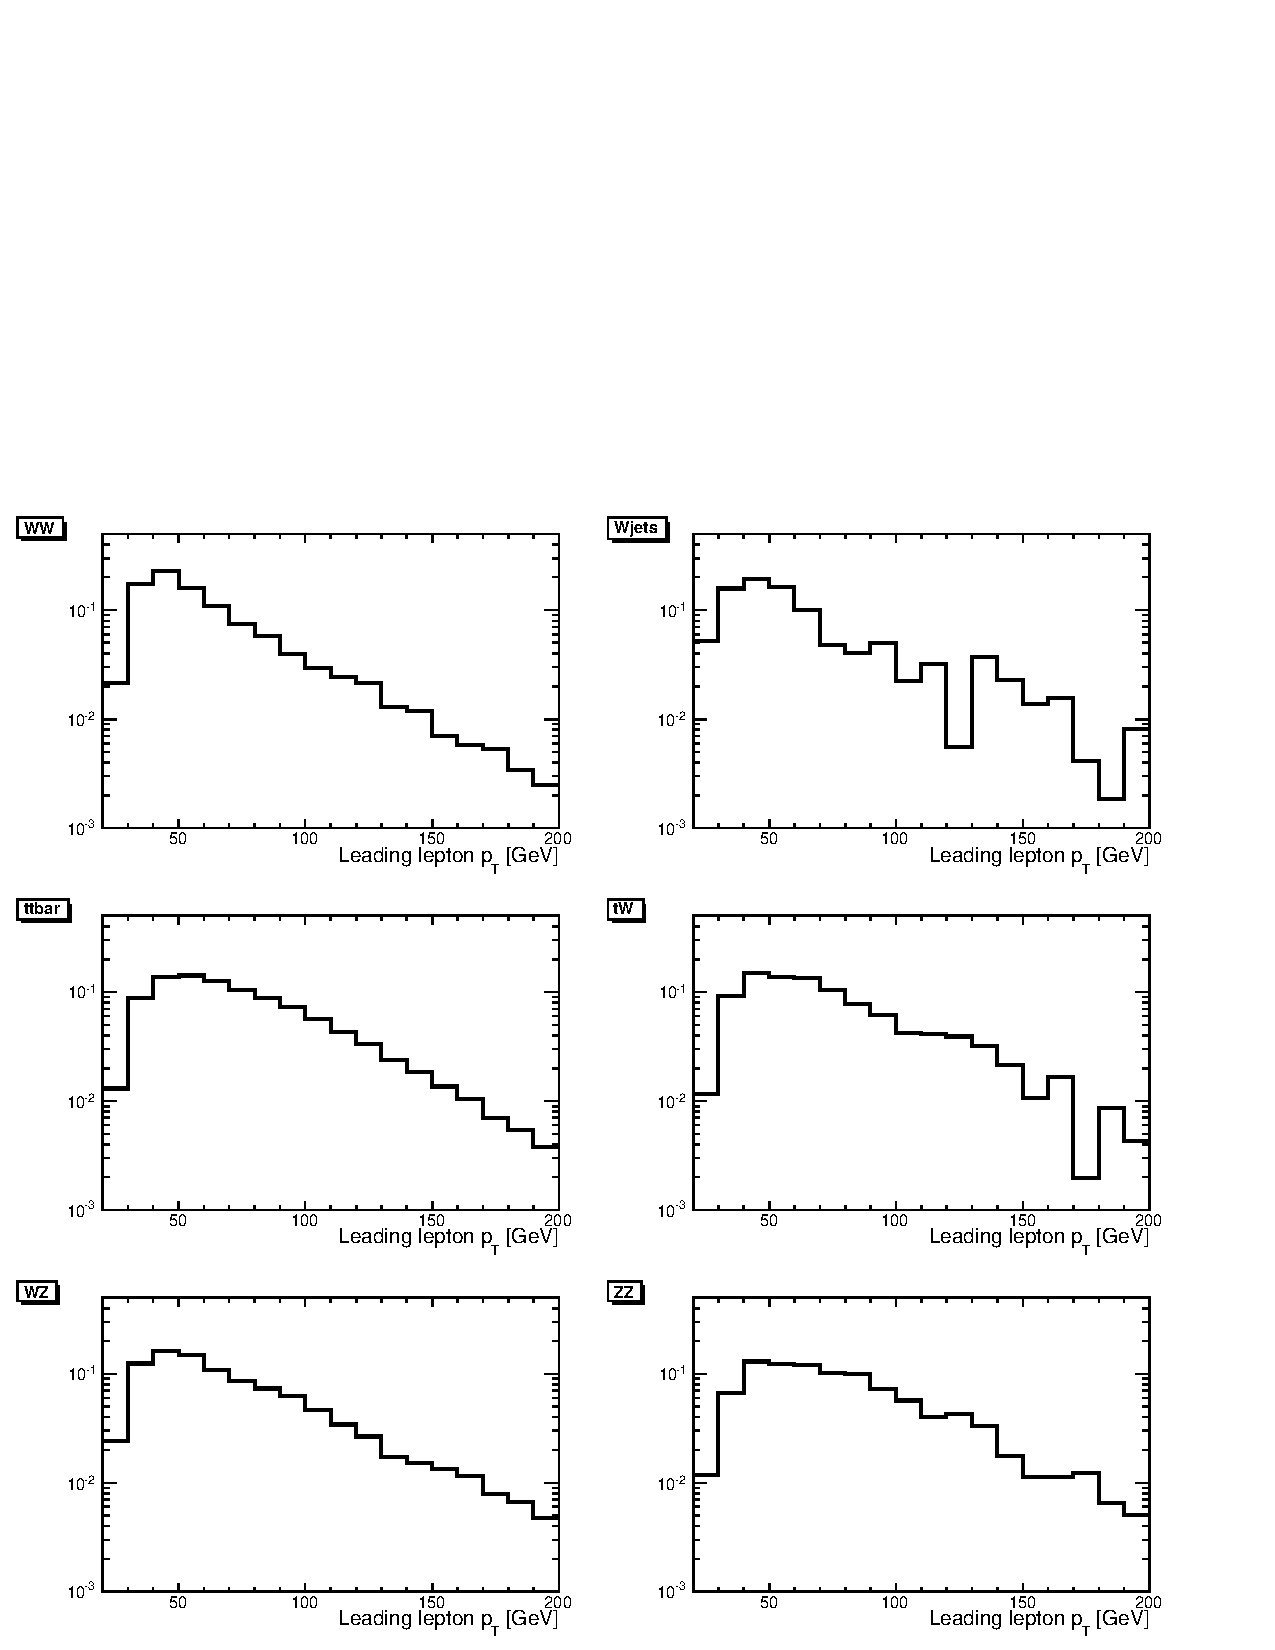
\includegraphics[width=0.7\textwidth]{figures/pdf_mc_all.pdf}
  }

  \caption[Background PDFs] {Leading lepton \pt\ PDFs for background
  events after full event selection.} \label{fig:bkgpdfs}
\end{figure}
